%%%%%%%%%%%%%%%%%%%%%%%%%%%%%%%%%%%%%%%%%%%%%%%%%%%%%%%%%%%%%%%%%%%%
\section{Relic density -- theoretical background}

%\index{relic density}

\subsection{The Boltzmann equation and thermal averaging}
\label{sec:Boltzmann}

Griest and Seckel \cite{Griest:1990kh} have worked out the Boltzmann
equation when coannihilations are included. We start by reviewing
their expressions and then continue by rewriting them into a more
convenient form that resembles the familiar case without
coannihilations. This allows us to use similar expressions for
calculating thermal averages and solving the Boltzmann equation
whether coannihilations are included or not. The implementation in
\ds\ is based upon the work done in \cite{Edsjo:1997bg}. 
%We will later in this
%chapter, for the sake of clarification, assume that we work with
%supersymmetric dark matter with the lightest neutralino being the
%LSP. The routines here are completely general though and the interface
%between supersymmetry and the relic density routines is handled by the
%routines in \codeb{src/rn}.


\subsection{Review of the Boltzmann equation with coannihilations}
\label{RD:review}
%\index{Boltzmann equation}
Consider annihilation of $N$ DM particles $\chi_i$
($i=1,\ldots,N$) with masses $m_i$ and internal degrees of freedom
(statistical weights) $g_i$.  Also assume that $m_1 \leq m_2 \leq
\cdots \leq m_{N-1} \leq m_N$ and that $R$-parity is conserved. Note
that for the mass of the lightest stable of the particles we will use the
notation $m_{\chi}$ and $m_{1}$ interchangeably.

The evolution of the number density $n_i$ of particle $i$ is
\begin{eqnarray} \label{eq:Boltzmann}
  \frac{dn_{i}}{dt} 
  &=& 
  -3 H n_{i} 
  - \sum_{j=1}^N \langle \sigma_{ij} v_{ij} \rangle 
    \left( n_{i} n_{j} - n_{i}^{\rm{eq}} n_{j}^{\rm{eq}} \right) 
  \nonumber \\ 
  & & 
  - \sum_{j\ne i} 
  \big[ \langle \sigma'_{Xij} v_{ij} \rangle 
        \left( n_i n_X - n_{i}^{\rm{eq}} n_{X}^{\rm{eq}} \right)
      - \langle \sigma'_{Xji} v_{ij} \rangle
        \left( n_j n_X - n_{j}^{\rm{eq}} n_{X}^{\rm{eq}} \right)
  \big]
  \nonumber \\ 
  & &
  - \sum_{j\ne i} 
  \big[ \Gamma_{ij} 
        \left( n_i - n_i^{\rm{eq}} \right) 
      - \Gamma_{ji} 
        \left( n_j - n_j^{\rm{eq}} \right) 
  \big] .
\end{eqnarray}
The first term on the right-hand side is the dilution due to the
expansion of the Universe. $H$ is the Hubble parameter. The second
term describes $\chi_i\chi_j$ annihilations, whose total
annihilation cross section is 
\begin{eqnarray}
  \sigma_{ij}  & = & \sum_X \sigma (\chi_i \chi_j \rightarrow X).
\end{eqnarray}
The third term describes $\chi_i \to \chi_j$ conversions by
scattering off the cosmic thermal background,
\begin{eqnarray}
  \sigma'_{Xij} & = & \sum_Y \sigma (\chi_i X \rightarrow \chi_j Y)
\end{eqnarray}
being the inclusive scattering cross section. The last term accounts
for $\chi_i$ decays, with inclusive decay rates 
\begin{eqnarray}
  \Gamma_{ij}  & = & \sum_X \Gamma (\chi_i \rightarrow \chi_j X).
\end{eqnarray}
In the previous expressions, $X$ and $Y$
are (sets of) standard model particles involved in the
interactions, $v_{ij}$ is the `relative velocity' defined by
\begin{equation}
  v_{ij} = \frac{\sqrt{(p_{i} \cdot p_{j})^2-m_{i}^2 m_{j}^2}}{E_{i} E_{j}}
\end{equation}
with $p_{i}$ and $E_{i}$ being the four-momentum and energy of 
particle $i$, and finally $n_{i}^{\rm{eq}}$ is the equilibrium number
density of particle $\chi_i$,
\begin{equation}
  n_{i}^{\rm{eq}} = \frac{g_{i}}{(2\pi)^3} \int d^3{\bf p}_{i}f_{i}
\end{equation}
where ${\bf p}_i$ is the three-momentum of particle $i$, and
 $f_i$ is its equilibrium distribution function. 
In the Maxwell-Boltzmann approximation it is given by
\begin{equation}
  f_{i} = e^{-E_{i}/T}.
\end{equation}
The thermal average $\langle\sigma_{ij}v_{ij}\rangle$ is defined
with equilibrium distributions and is given by
\begin{equation}
  \langle \sigma_{ij}v_{ij} \rangle = \frac{\int d^3{\bf
      p}_{i}d^3{\bf p}_{j} 
  f_{i}f_{j}\sigma_{ij}v_{ij}}
  {\int d^3{\bf p}_{i}d^3{\bf p}_{j}f_{i}f_{j}}
\end{equation}

Normally, the decay rate of particles $\chi_i$ other
than the lightest which is stable is much faster than the age of the
universe. Since we have assumed $R$-parity conservation, all of these
particles decay into the lightest one. So its final abundance is
simply described by the sum
\begin{equation}
  n= \sum_{i=1}^N n_{i}.
\end{equation}
For $n$ we get the following evolution equation
\begin{equation}
  \frac{dn}{dt} = -3Hn - \sum_{i,j=1}^N \langle \sigma_{ij} v_{ij} \rangle 
  \left( n_{i}n_{j} - n_{i}^{\rm{eq}}n_{j}^{\rm{eq}} \right)
\end{equation}
where the terms on the second and third lines in
Eq.~(\ref{eq:Boltzmann}) cancel in the sum. 

The scattering rate of DM particles off particles in the
thermal background is much faster than their annihilation rate,
because the scattering cross sections $\sigma'_{Xij}$ are of the same
order of magnitude as the annihilation cross sections $\sigma_{ij}$
but the background particle density $n_X$ is much larger than each of
the DM particle densities $n_i$ when the former are
relativistic and the latter are non-relativistic, and so suppressed by
a Boltzmann factor. In this case, the $\chi_i$ distributions remain in
thermal equilibrium, and in particular their ratios are equal to the
equilibrium values,
\begin{equation}
  \frac{n_{i}}{n} \simeq \frac{n_{i}^{\rm{eq}}}{n^{\rm{eq}}}.
\end{equation}
We then get
\begin{equation} \label{eq:Boltzmann2}
  \frac{dn}{dt} =
  -3Hn - \langle \sigma_{\rm{eff}} v \rangle 
  \left( n^2 - n_{\rm{eq}}^2 \right)
\end{equation}
where
\begin{equation} \label{eq:sigmaveffdef}
  \langle \sigma_{\rm{eff}} v \rangle = \sum_{ij} \langle
  \sigma_{ij}v_{ij} \rangle \frac{n_{i}^{\rm{eq}}}{n^{\rm{eq}}}
  \frac{n_{j}^{\rm{eq}}}{n^{\rm{eq}}}.
\end{equation}

%%%%%%%%%%%%%%%%%

\subsection{Thermal averaging}
\label{sec:thermav}

%\index{thermal average}
So far the reviewing. Now let's continue
by reformulating the thermal averages into
more convenient expressions. 

We rewrite Eq.~(\ref{eq:sigmaveffdef}) as
\begin{equation} \label{eq:sigmaveff}
  \langle \sigma_{\rm{eff}} v \rangle = \frac{ \sum_{ij} \langle
  \sigma_{ij}v_{ij} \rangle n_{i}^{\rm{eq}} n_{j}^{\rm{eq}}}{n^2_{\rm{eq}}}
  = 
  \frac{A}{n_{\rm{eq}}^2} \, .
\end{equation}

For the denominator we obtain, 
using Boltzmann statistics for $f_i$,
\begin{equation} \label{eq:neq}
  n^{\rm eq} = \sum_i n^{\rm eq}_i = 
  \sum_i \frac{g_i}{(2\pi)^3} \int d^3 p_i 
  e^{-E_{i}/T} = 
  \frac{T}{2\pi^2} \sum_i g_i m_{i}^2
  K_{2} \left( \frac{m_{i}}{T}\right)
\end{equation}
where $K_{2}$ is the modified Bessel function of the second kind of 
order 2.

The numerator is the total annihilation rate per unit volume
at temperature $T$,
\begin{equation} 
  A = \sum_{ij} \langle \sigma_{ij} v_{ij} \rangle n_i^{\rm eq}
  n_j^{\rm eq} = \sum_{ij} \frac{g_{i}g_{j}}{(2\pi)^6} \int d^3 {\bf p}_{i}
  d^3{\bf p}_{j} f_{i}f_{j} \sigma_{ij} v_{ij}
\end{equation}
It is convenient
to cast it in a covariant form,
\begin{equation} 
  A = \sum_{ij} 
  \int W_{ij} \frac{g_i f_i d^3{\bf p}_i}{(2\pi)^3 2E_i}
  \frac{g_j f_j d^3{\bf p}_j}{(2\pi)^3 2E_j} .
\label{eq:Aij2}
\end{equation}
$W_{ij}$ is the (unpolarized) annihilation rate per unit volume
corresponding to the covariant normalization of $2E$ colliding
particles per unit volume. $W_{ij}$ is a dimensionless Lorentz
invariant, related to the (unpolarized) cross section
through\footnote{The quantity $w_{ij}$ in Ref.\ \protect\cite{Srednicki:1988ce}
  is $W_{ij}/4$.}
\begin{equation} \label{eq:Wijcross}
  W_{ij} = 4 p_{ij} \sqrt{s} \sigma_{ij} = 4 \sigma_{ij} \sqrt{(p_i
\cdot p_j)^2 - m_i^2 m_j^2} = 4 E_{i} E_{j} \sigma_{ij} v_{ij} .
\end{equation}
Here
\begin{equation}
  p_{ij} =
\frac{\left[s-(m_i+m_j)^2\right]^{1/2}
\left[s-(m_i-m_j)^2\right]^{1/2}}{2\sqrt{s}}
\end{equation}
is the momentum of particle $\chi_i$ (or $\chi_j$) in the
center-of-mass frame of the pair $\chi_i\chi_j$.

Averaging over initial and summing over final internal states, the
contribution to $W_{ij}$ of a general $n$-body final state is
\begin{equation}
  W^{n\rm{-body}}_{ij} = 
  \frac{1}{g_i g_j S_f} \sum_{\rm{internal~d.o.f.}} 
  \int  \left| {\cal M} \right|^2 (2\pi)^4 
\delta^4(p_i+p_j-{\textstyle \sum_f}p_f) \prod_f
   \frac{d^3{\bf p}_f}{(2\pi)^3 2E_f} , 
\end{equation}
where $S_f$ is a symmetry factor accounting for identical final state
particles (if there are $K$ sets of $N_k$ identical particles,
$k=1,\dots,K$, then $S_f = \prod_{k=1}^{K} N_k!$).  In particular, 
the contribution
of a two-body final state can be written as
\begin{equation}
  W^{\rm{2-body}}_{ij\to kl} = \frac{p_{kl}}{16\pi^2 g_i g_j S_{kl} \sqrt{s}}
  \sum_{\rm{internal~d.o.f.}} \int \left| {\cal M}(ij\to kl) \right|^2
  d\Omega ,
\end{equation}
where $p_{kl}$ is the final center-of-mass momentum, $S_{kl}$ is a
symmetry factor equal to 2 for identical final particles and to 1
otherwise, and the integration is over the outgoing directions of
one of the final particles.  As usual, an average over initial
internal degrees of freedom is performed.

We now reduce the integral in the covariant expression for $A$,
Eq.~(\ref{eq:Aij2}), from 6 dimensions to 1.
Using Boltzmann statistics for $f_i$ (a good approximation for
$T\lsim m$)
\begin{equation} \label{eq:Aij2b}
  A =
  \sum_{ij} \int g_i g_j W_{ij} e^{-E_{i}/T} e^{-E_{j}/T} 
\frac{d^3{\bf p}_i}{(2\pi)^3 2E_i}
  \frac{d^3{\bf p}_j}{(2\pi)^3 2E_j} ,
\end{equation}
where ${\bf p}_{i}$ and ${\bf p}_{j}$ are the three-momenta and
$E_{i}$ and $E_{j}$ are the energies of the colliding particles.
Following the procedure in Ref.~\cite{Gondolo:1990dk} we then rewrite
the momentum volume element as
\begin{equation}
  d^3 {\bf p}_{i} d^3 {\bf p}_{j} = 4 \pi |{\bf p}_{i}| E_i dE_{i}
  \, 4 \pi |{\bf p}_{j}| E_j dE_{j} \, \frac{1}{2} d \cos \theta
\end{equation}
where $\theta$ is the angle between ${\bf p}_{i}$ and 
${\bf p}_{j}$. Then we change integration variables from 
$E_{i}$, $E_{j}$, $\theta$ to $E_{+}$, $E_{-}$ and $s$, given by
\begin{equation}
  \left\{ \begin{array}{lcl}
  E_{+} & = & E_{i}+E_{j} \\
  E_{-} & = & E_{i}-E_{j} \\
  s & = & m_{i}^2+m_{j}^2 + 2E_{i}E_{j}-2 |{\bf p}_{i}| |{\bf
    p}_{j}| \cos \theta,
  \end{array} \right.
\end{equation}
whence the volume element becomes
\begin{equation}
  \frac{d^3{\bf p}_i}{(2\pi)^3 2E_i} \frac{d^3{\bf p}_j}{(2\pi)^3 2E_j} =
  \frac{1}{(2\pi)^4} \frac{dE_{+}dE_{-}ds}{8},
\end{equation}
and the integration region $\{ E_i \geq m_i, E_j \geq m_j, |\cos \theta| 
\leq
1\}$ transforms into 
\begin{eqnarray}
  && s \geq (m_i+m_j)^2, \\ && E_{+} \geq \sqrt{s} , \\ && \left\vert
  E_{-} - E_{+} \frac{m_j^2-m_i^2}{s} \right\vert \leq 2 p_{ij}
  \sqrt{\frac{E_{+}^2-s}{s}}.
\end{eqnarray}

Notice now that the product of the equilibrium distribution
functions depends only on $E_{+}$ and not $E_{-}$ due to the
Maxwell-Boltzmann approximation, and that the invariant rate
$W_{ij}$ depends only on $s$ due to the neglect of final state
statistical factors. Hence we can immediately integrate over
$E_{-}$,
\begin{equation}
  \int dE_{-} = 4p_{ij} \sqrt{\frac{E_{+}^2-s}{s}}.
\end{equation}
The volume element is now
\begin{equation}
  \frac{d^3{\bf p}_i}{(2\pi)^3 2E_i} \frac{d^3{\bf p}_j}{(2\pi)^3 2E_j} = 
  \frac{1}{(2\pi)^4} \frac{p_{ij}}{2} \sqrt{\frac{E_{+}^2-s}{s}} 
dE_{+} ds 
\end{equation}

We now perform the $E_{+}$ integration. We obtain
\begin{equation}
\label{eq:As}
  A = \frac{T}{32 \pi^4} \sum_{ij} \int_{(m_i+m_j)^2}^\infty ds
  g_ig_jp_{ij} W_{ij} K_{1} \left( \frac{\sqrt{s}}{T}\right)
\end{equation}
where $K_{1}$ is the modified Bessel function of the second kind of 
order 1.

We can take the sum inside the integral and define an effective
annihilation rate $W_{\rm eff}$ through
\begin{equation}
  \sum_{ij} g_i g_j p_{ij} W_{ij} = g_1^2 p_{\rm{eff}} W_{\rm{eff}}
\end{equation}
with
\begin{equation}
\label{eq:peff}
  p_{\rm{eff}} = p_{11} = \frac{1}{2} \sqrt{s-4m_{1}^2} .
\end{equation}
In other words
\begin{equation} \label{eq:weff}
  W_{\rm{eff}} = \sum_{ij}\frac{p_{ij}}{p_{11}}
  \frac{g_ig_j}{g_1^2} W_{ij} = 
  \sum_{ij} \sqrt{\frac{[s-(m_{i}-m_{j})^2][s-(m_{i}+m_{j})^2]}
  {s(s-4m_1^2)}} \frac{g_ig_j}{g_1^2} W_{ij}.
\end{equation}
Because $W_{ij}(s) = 0 $ for $s \le (m_i+m_j)^2$, the radicand is  
never negative.

In terms of cross sections, this is equivalent to the definition
\begin{equation}
\sigma_{\rm eff} = \sum_{ij} \frac{p^2_{ij}}{p^2_{11}}
  \frac{g_ig_j}{g_1^2} \sigma_{ij}.
\end{equation}  

Eq.~(\ref{eq:As}) then reads
\begin{equation}
  A = \frac{g_1^2 T}{32 \pi^4} \int_{4m_1^2}^\infty ds
  p_{\rm eff} W_{\rm eff} K_{1} \left( \frac{\sqrt{s}}{T}\right)
\end{equation}
This can be written in a form more suitable
for numerical integration by using $p_{\rm{eff}}$ instead of $s$ as
integration variable.  From Eq.~(\ref{eq:peff}), we have 
 $ ds = 8 p_{\rm{eff}} dp_{\rm{eff}} $, and 
\begin{equation}
\label{eq:Apeff}
  A = \frac{g_1^2 T}{4 \pi^4} \int_{0}^\infty dp_{\rm eff}
  p^2_{\rm eff} W_{\rm eff} K_{1} 
  \left( \frac{\sqrt{s}}{T}\right)
\end{equation}
with
\begin{equation}
  s = 4p_{\rm{eff}}^2 + 4m_1^2
\end{equation}
So we have succeeded in rewriting $A$ as a 1-dimensional integral.

{}From Eqs.~(\ref{eq:Apeff}) and~(\ref{eq:neq}), the thermal average of
the effective cross section results
\begin{equation} \label{eq:sigmavefffin2}
  \langle \sigma_{\rm{eff}}v \rangle = \frac{\int_0^\infty
  dp_{\rm{eff}} p_{\rm{eff}}^2 W_{\rm{eff}} K_1 \left(
  \frac{\sqrt{s}}{T} \right) } { m_1^4 T \left[ \sum_i \frac{g_i}{g_1}
  \frac{m_i^2}{m_1^2} K_2 \left(\frac{m_i}{T}\right) \right]^2}.
\end{equation}
This expression is very similar to the case without coannihilations,
the differences being the denominator and the replacement of the
annihilation rate with the effective annihilation rate. 
In the absence of coannihilations, this expression
correctly reduces to the formula in Gondolo and
Gelmini~\cite{Gondolo:1990dk}.

The definition of an effective annihilation rate independent of
temperature is a remarkable calculational advantage. As in the case
without coannihilations, the effective annihilation rate can in fact
be tabulated in advance, before taking the thermal average and
solving the Boltzmann equation.

\begin{figure}
  \centerline{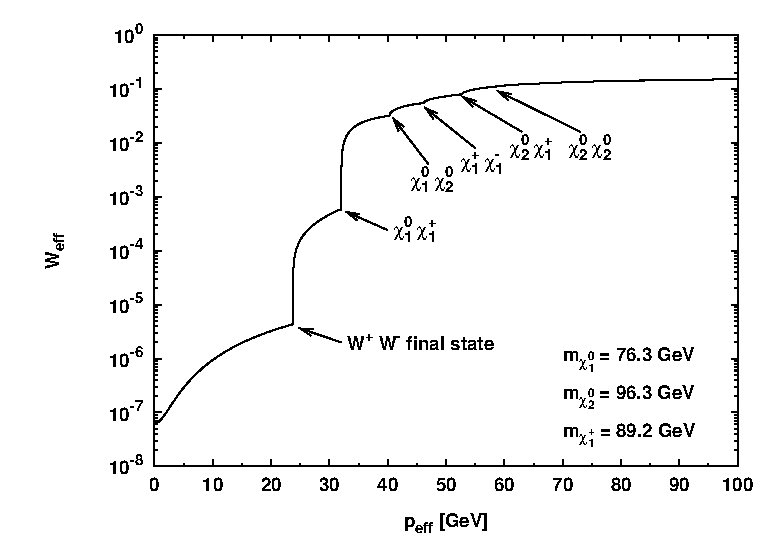
\epsfig{file=fig/rateex.eps,width=0.75\textwidth}}
  \caption{The effective invariant annihiliation rate $W_{\rm eff}$
    as a function of $p_{\rm eff}$ for an example \code{mssm} model. 
    The final state threshold for
    annihilation into $W^+ W^-$ and the coannihilation thresholds, as
    given by Eq.~(\protect\ref{eq:weff}), are indicated.  
    The $\chi_2^0 \chi_2^0$ coannihilation threshold is too small to
    be seen.}
  \label{fig:effrate}
\end{figure}

In the effective annihilation rate, coannihilations appear
as thresholds at $\sqrt{s}$ equal to the sum of the masses of the
coannihilating particles.  We show an example for neutralino
DM (in the \code{mssm} module) in
Fig.~\ref{fig:effrate} where it is clearly seen that the
coannihilation thresholds appear in the effective invariant rate
just as final state thresholds do.  For the same example,
Fig.~\ref{fig:k1effrate} shows the differential annihilation rate
per unit volume $dA/dp_{\rm eff}$, the integrand in
Eq.~(\ref{eq:Apeff}), as a function of $p_{\rm eff}$. We have
chosen a temperature $T=m_{\chi}/20$, a typical freeze-out
temperature. The Boltzmann suppression contained in the exponential
decay of $K_{1}$ at high $p_{\rm eff}$ is clearly visible.  At
higher temperatures the peak shifts to the right and at lower
temperatures to the left.  For the particular model shown in
Figs.~\ref{fig:effrate}--\ref{fig:k1effrate}, the relic density
results $\Omega_\chi h^2=0.030$ when coannihilations are included
and $\Omega_\chi h^2=0.18$ when they are not. Coannihilations
have lowered $\Omega_\chi h^2$ by a factor of 6.

\begin{figure}
  \centerline{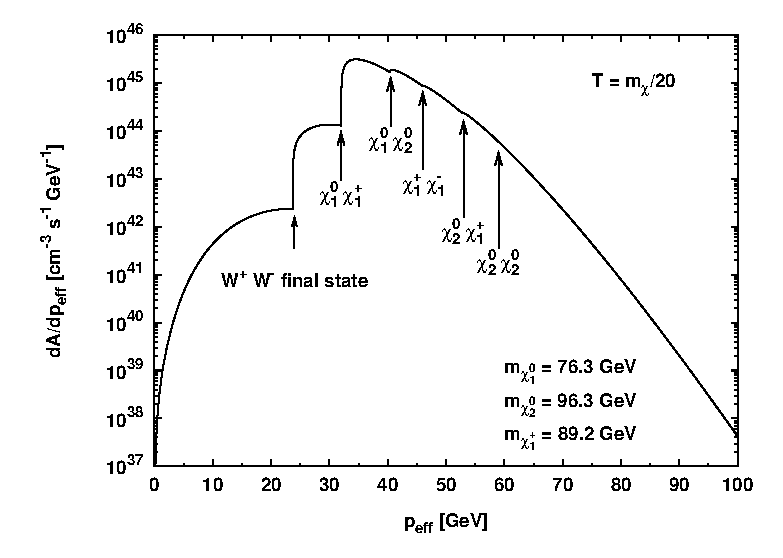
\epsfig{file=fig/k1rateex.eps,width=0.75\textwidth}}
  \caption{Total differential annihilation rate per unit volume 
    $dA/dp_{\rm eff}$ for the same model as in
    Fig.~\protect\ref{fig:effrate}, evaluated at a temperature
    $T=m_\chi/20$, typical of freeze-out. Notice the Boltzmann
    suppression at high $p_{\rm eff}$.}
  \label{fig:k1effrate}
\end{figure}



%%%%%%%%%%%%%%%%%%%%%%%%%%%%%%%%%%%%%%
\subsection{Reformulation of the Boltzmann equation}

%\index{Boltzmann equation}
We now follow Gondolo and Gelmini \cite{Gondolo:1990dk} to 
put Eq.~(\ref{eq:Boltzmann2}) in a more convenient form by
considering the ratio of the number density to the entropy density,
\begin{equation} \label{eq:ydef}
  Y = \frac{n}{s}.
\end{equation}
Consider
\begin{equation}
  \frac{dY}{dt} = \frac{d}{dt} \left( \frac{n}{s} \right) = 
  \frac{\dot{n}}{s}-\frac{n}{s^2}\dot{s}
\end{equation}
where dot means time derivative. In absence
of entropy production, $S=R^3s$ is constant ($R$ is the scale factor).
Differentiating with respect to time we see 
that
\begin{equation}
  \dot{s} = -3\frac{\dot{R}}{R} s = -3Hs
\label{eq:entropycons}
\end{equation}
which yields
\begin{equation}
  \dot{Y} = \frac{\dot{n}}{s} + 3H \frac{n}{s}.
\end{equation}
Hence we can rewrite Eq.~(\ref{eq:Boltzmann2}) as
\begin{equation} \label{eq:Boltzmann3}
  \dot{Y} = -s  \langle \sigma_{\rm{eff}} v \rangle 
  \left( Y^2 - Y_{\rm{eq}}^2 \right).
\end{equation}

The right-hand side depends only on temperature, and it is therefore
convenient to use temperature $T$ instead of time $t$ as independent
variable. Defining $x=m_1/T$ we have
\begin{equation}
  \frac{dY}{dx} = - \frac{m_{1}}{x^2} \frac{1}{3H} \frac{ds}{dT}
  \langle \sigma_{\rm{eff}} v \rangle \left( Y^2 -
  Y_{\rm{eq}}^2 \right).
\label{eq:Boltzmann3bis}
\end{equation}
where we have used
\begin{equation}
  \frac{1}{\dot{T}} = \frac{1}{\dot{s}} \frac{ds}{dT} = -
  \frac{1}{3Hs} \frac{ds}{dT} 
\end{equation} 
which follows from Eq.~(\ref{eq:entropycons}). 
With the Friedmann equation in a radiation dominated universe
\begin{equation}
  H^2 = \frac{8\pi G \rho}{3} ,
\end{equation}
where $G$ is the gravitational constant, and the
usual parameterization of the energy and entropy densities
in terms of the effective degrees of freedom $g_{\rm{eff}}$ and
$h_{\rm{eff}}$, \begin{equation} \label{eq:geffheff}
  \rho = g_{\rm{eff}}(T) \frac{\pi^2}{30} T^4
  , \quad 
  s = h_{\rm{eff}}(T) \frac{2\pi^2}{45} T^3 ,
\end{equation}
we can cast Eq.~(\ref{eq:Boltzmann3bis})
into the form \cite{Gondolo:1990dk}
\begin{equation} \label{eq:Boltzmann4}
  \frac{dY}{dx} = - \sqrt{\frac{\pi}{45G}} \frac{g_{*}^{1/2}m_1}{x^2}
  \langle \sigma_{\rm{eff}} v \rangle \left( Y^2 -
  Y_{\rm{eq}}^2 \right) 
\end{equation}
where $Y_{\rm eq}$ can be written as
\begin{equation}
  Y_{\rm{eq}} = \frac{n_{\rm{eq}}}{s} = 
  \frac{45 x^2}{4 \pi^4 h_{\rm{eff}}(T)} \sum_i g_i
  \left( \frac{m_i}{m_1} \right)^2 K_{2} \left( x 
\frac{m_{i}}{m_1}\right),
\end{equation}
using Eqs.~(\ref{eq:neq}), (\ref{eq:ydef}) and
(\ref{eq:geffheff}).

The parameter $g_{*}^{1/2}$ is defined as
\begin{equation}
  g_{*}^{1/2} = \frac{h_{\rm{eff}}}{\sqrt{g_{\rm{eff}}}}
  \left( 1+\frac{T}{3h_{\rm{eff}}} \frac{d h_{\rm{eff}}}{dT}
  \right)
\end{equation}

For $g_{\rm eff}$, $h_{\rm eff}$ and $g_*^{1/2}$, the user can choose different implementations by a call to 
the routine \code{dsrdset} (see that routine for further details). The default for those effective relativistic 
degrees of freedom is to use the results from Drees et al \cite{Drees:2015exa}.

%Our results are insensitive to the
%value of $T_{QCD}$, because due to a lower limit on the neutralino
%mass the neutralino freeze-out temperature is always much larger
%than $T_{QCD}$.

To obtain the relic density we integrate Eq.~(\ref{eq:Boltzmann4})
from $x=0$ to $x_0=m_\chi/T_0$ where $T_0$ is the photon temperature
of the Universe today. The relic density today in units of the
critical density is then given by
\begin{equation}
  \Omega_\chi = \rho_\chi^0/\rho_{\rm
  crit}=m_\chi s_0 Y_0/\rho_{\rm crit}
\end{equation}
where $\rho_{\rm crit}=3 H^2/8 \pi G$ is the critical density, $s_{0}$ 
is the entropy density today and $Y_{0}$ is the result of the 
integration of Eq.~(\ref{eq:Boltzmann4}). With a
background radiation temperature of $T_0=2.726$ K we finally obtain
\begin{equation} \label{eq:omegah2}
  \Omega_\chi h^2 = 2.755\times 10^8 \frac{m_\chi}{\mbox{GeV}} Y_0.
\end{equation}
